\documentclass[12pt,a4paper]{report}
\usepackage{fullpage}
\usepackage[left=2cm,right=2cm,top=2cm,bottom=2cm]{geometry}

\usepackage[pdftex]{graphicx}
\usepackage[dvipsnames]{xcolor}
\usepackage{wrapfig}
\usepackage{mwe}
\usepackage{subcaption}
\usepackage{amsmath}

\setlength{\parindent}{1cm}
\setlength{\parskip}{1ex plus 0.5ex minus 0.2ex}
\newcommand{\hsp}{\hspace{20pt}}
\newcommand{\HRule}{\rule{\linewidth}{0.5mm}}
%%%%%%%%%%%%%%%%%%%%%%%%%%%%%%%%%%%%%%%%%%%%%
\title{Rapport de projet Minimal Learning Machine}

\begin{document}
\begin{titlepage}
  \begin{sffamily}
  \begin{center}

    \textsc{\LARGE Université de Rouen}\\[2cm]

    \textsc{\Large Rapport de projet}\\[1.5cm]

    % Title
    \HRule \\[0.4cm]
    { \huge \bfseries Minimal Learning Machine \\[0.4cm] }

    \HRule \\[2cm]
    
\includegraphics[scale=0.2]{SID.png}
    \\[2cm]

    % Author and supervisor
    \begin{minipage}{0.4\textwidth}
      \begin{flushleft} \large
       Étudiant\\Encadrant
      \end{flushleft}
    \end{minipage}
    \begin{minipage}{0.4\textwidth}
      \begin{flushright} \large
      Laziz Hamdi\\M. Simon Bernard
      \end{flushright}
    \end{minipage}

    \vfill

    % Bottom of the page
    {\large 2020 — 2021}

  \end{center}
  \end{sffamily}
\end{titlepage}
%%%%%%%%%%%%%%%%%%%%%%%% document %%%%%%%%%%%%%%%%%%
\thispagestyle{empty}
\chapter*{Remerciements}
\addcontentsline{toc}{chapter}{Remerciements}
\par \textit{Il était agréable de m'acquitter d'une dette de reconnaissance envers tous ceux, dont la contribution au cours de ce projet, a favorisé son aboutissement. \\\\
 Ainsi je tiens vivement à remercier mon encadrant Mr Simon Bernard qui n'a pas ménagé aucun effort pour m'aider et m'orienter le long de ce projet, merci Mr Simon Bernard. Je remercie aussi le professeur Mr Maxime Berar pour son  encadrement et le soutien qu'il m'a donné.\\\\
 Je remercie enfin toute personne qui a contribué de près ou de loin à l'élaboration de ce rapport. 
}

\tableofcontents
{\color{MidnightBlue}\chapter{Introduction}}

\par En apprentissage automatique on distingue deux principales situations, dans le cas où les données à prédire ne sont pas étiquetés ce que l'on appelle l'apprentissage non supervisé. Dans le cas contraire lorsque les données à prédire sont étiquetés on appelle ça apprentissage supervisé. Il existe des tas de méthodes d'apprentissage supervisé parmi les plus connues on a les SVM (Support Vector Machine) ou encore RF (Random Forest). Il existe une technique qui est souvent utilisé en machine learning dans différentes tâches tel que la réduction de dimension, cette technique est l'utilisation d'une mesure de similarité ou dissimilarité entre les données.

\par Il existe plusieurs moyens de calculer une similiarité ou dissimilarité entre les données, le moyen le plus connue est sans doute les distances. Dans ce rapport je vous présente une méthode d'apprentissage supervisé qui se base sur le calcul de dissimilarité entre les données en utilisant les distances. Il s'agit du Minimal Learning Machine ou MLM. Ce document se divise en trois parties principales, chaque partie présente l'un des objectifs de ce TER qui sont dans un premier temps de comprendre et de documenter la méthode ensuite de reprendre les expérimentations présentées dans les articles du MLM pour ensuite implémenter une version de la méthode de référence qui serait "kernelizable" ou "pré calculé" et de tester cette version avec des Random Forest. 

{\color{MidnightBlue}\chapter{Minimal Learning Machine}}
{\color{MidnightBlue}\section{Définition}}
\par Le Minimal Learning Machine est une technique d'apprentissage supervisé apparu en 2015 qui fonctionne sur des problèmes de régressions ou de classifications. Dans sa phase d'entraînement, les données sont projetées dans un nouvel espace. Pour cela des observations aléatoires sont sélectionnées depuis les données, ensuite des distances qu'on appellera \textbf{"dissimilarités"} sont calculées entre ces observations et l'ensemble des données. Dans ce nouvel espace on ne cherche plus à prédire les mêmes données mais plutôt à prédire des distances.\ 
Et une fois ces distances prédites, on utilise le processus inverse pour estimer les réelles valeurs.\
{\color{MidnightBlue}\section{Phase d'entraînement}}
{\color{MidnightBlue}\subsection{Formulation}}
\par Pour un ensemble de données en entrée $X = \{x_i\}_{i=1}^{N}$ avec
$x_i \in R$ et sa correspondance en sortie $Y = \{y_i\}_{i=1}^{N}$ avec $y_i \in S$.\\
On suppose qu'il existe une relation continue entre ces deux espaces qu'on appelle $f: X \rightarrow Y$, l'objectif est d'estimer $f$.\\
Le processus du MLM se divise en deux étapes principales:\\\\
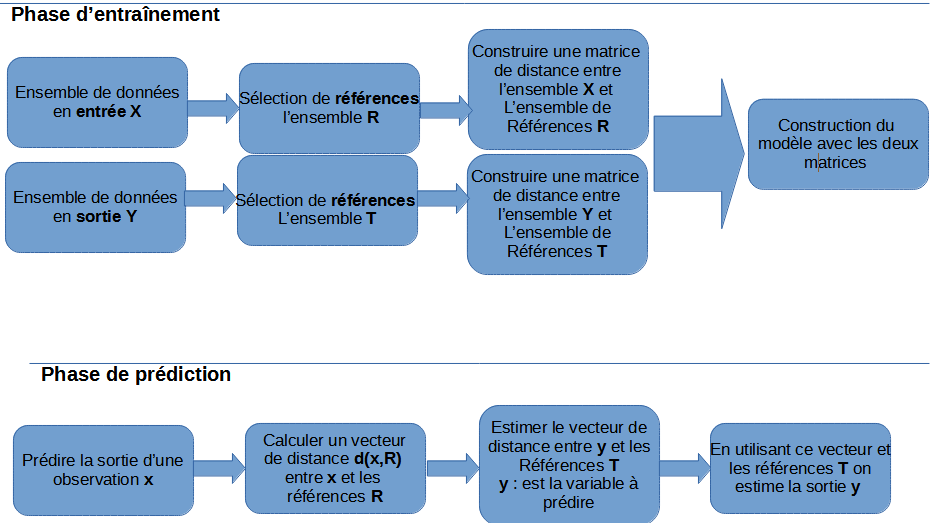
\includegraphics[scale=0.72]{schema.png}

{\color{MidnightBlue}\subsection{Construire les matrices de distances}}
\par Le MLM requière que l'utilisateur précise le nombre de points références $k$ à sélectionner pour construire ce qu'on appelle des matrices de distances ou de dissimilarités.\
Si on considère $D$ une matrice de distance de taille $n,m$, la valeur qui se trouve à l'intersection de la ligne $i$ et la colonne $j$ représente la distance euclidienne entre l'observation $i$ et la référence $j$. De ce fait les lignes de $D$ représentent l'ensemble des observations et les colonnes l'ensemble des points références.\\
On définit l'ensemble des points références $R=\{m_k\}_{k=1}^k$ sélectionnés aléatoirement de l'ensemble $X$ et leurs correspondances $T =\{t_k\}_{k=1}^k$ de l'ensemble $Y$, ensuite on construit la matrice $D_x \in R^{N \times K}$ des distances euclidiennes entre les observations $x_i$ en ligne et les références  en colonne, de la même manière est définit la matrice des distances en sortie $\Delta_x \in R^{N \times K}$.\\
On définit la relation entre ces matrices ainsi $\Delta_y = g(D_x) + E$ avec E qui représente le résidu.\\
On peut représenter cette relation sous forme matricielle \boldmath{$\Delta_y = D_xB + E$}.\\$B$ est la matrice des coefficients du modèle.\\

{\color{MidnightBlue}\subsection{Construire le modèle}}
\par Pour estimer $B$ c'est à dire les coefficients du modèle, plusieurs méthodes peuvent être utiliser comme les moindres carrés moyens, moindres carrés récursifs pour calculer la différence entre les vraies distances et les distances prédites. cette différence est exprimé avec cette fonction.\\ \boldmath{$RSS(B) = tr((\Delta_y - D_xB)^\prime(\Delta_y - D_xB))$}\\
Minimiser cette fonction revient à chercher le point ou le gradient est null, ce qui conduit à résoudre un système d'équations ou le nombre d'équations est le nombre d'observations $N$ et le nombre d'inconnue est le nombre de références $K$. La solution est différente selon le nombre $K$.\\
\begin{itemize}
\item Pour $K < N$: \boldmath{$\hat{B} = ({D_x}^\prime D_x)^{-1} {D_x}^\prime \Delta_y$}
\item Pour $K = N$: \boldmath{$\hat{B} = {D_x}^{-1} \Delta_y$}
\item Pour $K > N$ : une infinité de solutions.
\end{itemize}

Ce dernier cas se produit lorsque après sélection des points références uniquement une partie des données est utilisé pour créer le modèle, ceci donne naissance à un problème indéterminé car le nombre d'équations est plus petit que le nombre d'inconnu avec une infinité de solution. 

{\color{MidnightBlue}\section{Phase de prédiction}}
\par Une fois $B$ estimer pour un point en entrée $x$, on construit un vecteur de distances euclidienne entre ce point et l'ensemble des point références $d(x,R) = [d(x,m_1)...d(x,m_k)]$, alors dans le cas ou $K = N$ ou $k < N$, le vecteur des distances en sortie est le produit entre le vecteur des distances en entrée et la matrice des coefficients.\\
$\hat{\delta}(y,T) = d(x,R)\hat{B}$ avec $\hat{\delta}(y,T) = [\hat{\delta}(y,t_1)...\hat{\delta}(y,t_k)]$

\par $y$ est estimé en utilisant le vecteur des distances $\hat{\delta}(y,T)$ et les références $T$ avec ce qu'on appelle une \textbf{multitaréation}. C'est une technique qui utilise des mesures de distance pour relever les coordonnées spatiales de positions inconnues. En pratique les distances sont mesurées avec erreur, et les méthodes statistiques peuvent quantifier l'incertitude de l'estimation de la position inconnue. De nombreuses méthodes d'estimation de la position d'un point par multitération peuvent être utiliser comme un estimateur linéaire des moindres carrés, un estimateur des moindres carrés pondéré de manières itérative et une technique non linéaire des moindres carrés. En général la technique des moindres carrés non linéaire est la plus performante.\\
Pour estimer $y$ on minimise la fonction objective suivante :\\
$\jmath(y) = \sum_{k-1}^{k}((y-t_k)\prime(y-t_k)-\hat{\delta}^2(y,t_k))^2$ \\
Cette fonction de coût possède un minimum en 0 qui est atteint seulement si la valeur estimer est égal à la vraie valeur, c'est à dire que les valeurs prédites sont égales aux  valeurs réels $\prime{y} = y$. Sinon on approche le plus possible $y$ avec un algorithme de minimisation. \\
\par Plusieurs algorithmes de minimisation peuvent être utilisés mais le plus adapter pour ce problème est L'algorithme de \textbf{Levenberg-Marquardt} qui permet de trouver une solution numérique à un problème de minimisation d'une fonction non linéaire dépendant de plusieurs variables. Cet algorithme est plus stable et trouve une solution même s'il démarre très loin du minimum. 

{\color{MidnightBlue}\section{Choix du paramètre K}}
\par Le principal avantage du MLM est qu'il ne possède qu'un seul hyper paramètre K à optimiser le nombre de points références que l'utilisateur doit rentrer. Pour optimiser le nombre de points références la validation croisée est utilisée, en divisant l'ensemble des données en F sous-ensembles ensuite en testant avec différentes valeurs de $k$ les taux de réussites sont calculés avec les moindres carrés moyens pour les vecteur de distances en sortie $\hat{\delta}$ et l'estimation des $\hat{y}$\\ \\
$AMSE(\delta) = \frac{1}{K} \sum_{k=1}^k \frac{1}{N_v} \sum_{i=1}^{N_v} (\delta(y_i,t_k) - \hat{\delta}(y_i,t_k))^2$ \\
$AMSE(y)=\frac{1}{4} \sum_{s = 1}^S \frac{1}{N_v} \sum_{i = 1}^{N_v} (y_i^{(s)} -\hat{y}_i^{(s)})^2$\\\\
Les points références sont sélectionnés aléatoirement des données. 

{\color{MidnightBlue}\section{Performances et Complexité}}
\par La complexité pour l'étape de formation du modèle  dépend fortement de la méthode utilisée pour le calcul des inversions de matrice surtout qu'on construit des matrices de distances toujours plus grandes selon la taille des données et le nombre de points références sélectionnées, puisque on construit des matrices de tailles $N,K$.\\
L'une des méthodes les plus connue est l'inverse de \textbf{Moore-Penrose} qui estime une pseudo inverse de la matrice, car dans certains cas les matrices ne sont pas inversibles. L'une des constructions les plus connues de cette méthode est la décomposition en valeurs singulières $SVD$ qui est très précise mais très gourmande en temps de calcule et est plusieurs fois plus élevé  que le produit matrice-matrice.\\
\par Pour accélérer le calcul, plusieurs méthodes ont été proposé comme le produit entre un type spécial de tenseur et une décomposition $QR$ ou encore un algorithme basé sur une factorisation \textbf{Cholesky}.\\
La complexité de la phase d'entrainement du MLM est $\Theta (K^2N)$ c'est similaire à celle d'un algorithme de machine learning lorsque le nombre de neurones cachés est égal au nombre de références K.

\par Le MLM est testé sur 12 ensembles de données les plus fréquemment utilisés dans le monde ensuite ces performances sont comparées à celle de cinq autre méthodes de références le machine learning, extrême learning machine \textbf{ELM}, le réseau de fonction à base radial \textbf{RBF}, les machines à vecteur de support \textbf{SVM}, les processus gaussiens \textbf{GP} et le percepteron multicouches \textbf{MLP}. Tous les ensembles de données sont près traités de la même manière pour reproduire les expériences à l'identique. Supprimer les données manquantes, supprimer les données catégorielles, normaliser de la même façon et utiliser la même proportion de données pour l'entraînement et le test. \\ \\
Pour ces tests le seul hyper paramètre K du MLM est optimisé avec une validation croisée sur 10-Fold, avec une sélection aléatoire des références depuis l'ensemble de données pour k allant de 5\% à 100\% avec un pas de 5\%. Tous les modèles sont évalués en utilisant l'erreur quadratique moyenne \textbf{MSE} sur 10 tests indépendants. Le MLM obtient le plus petit taux d'erreur pour 5/8 des problèmes de régressions et pour les autres problèmes il obtient des résultats proches des résultats obtenue par les autres méthodes.\\
Ces expériences montrent qu'en utilisant 20\% des points d'apprentissages comme points références semble être un bon choix pour la plupart des ensembles de données.

{\color{MidnightBlue}\chapter{Expérimentations}}
\par Pour évaluer les performances du Minimal Learning Machine, les chercheurs qui ont inventé la méthode ont comparé les résultats obtenus avec le MLM aux résultats obtenus avec les méthodes de machine learning les plus connus, sur 12 datasets, leur dimensions sont détaillés dans la table ci-dessous.
\begin{figure}[hbt!]
\centering
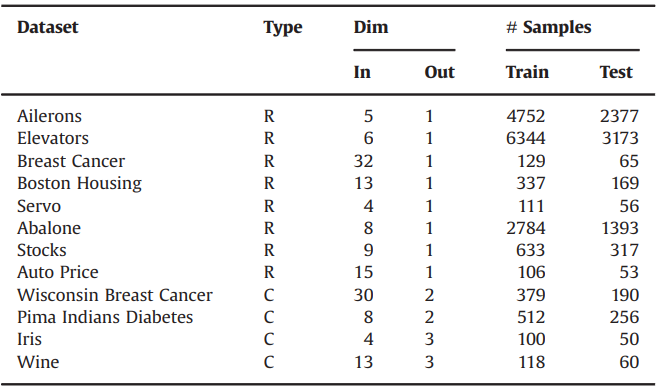
\includegraphics[scale=0.99]{data.png}
\end{figure}

\par Lors de ce projet on a reproduit certaines des expérimentations présentées dans l'article scientifique de la méthode sur 8/12 des précédents datasets n'ayant pas retrouvés les 4 autres.
\par On a suivi le même protocole pour tous les datasets, les données sont centrées et réduites avec la moyenne et écart type des données d’entraînements , les variables catégorielles ainsi que les instances qui contiennent des données manquantes sont supprimées. Dix différentes permutations aléatoires sont appliquées pour chaque dataset.2/3 de l'ensemble de données sont utilisés pour la phase d'entrainement du modèle et 1/3 pour la phase de test.\\
Il est a noté que pour la classification les proportions des classes ont été équilibré. Chaque classe est représentée avec une proportion égale pour la phase d'entrainement et de test.

\par Le seul hyper paramètre du Minimal Learning Machine c'est à dire le nombre de point référence, est optimisé avec une validation croisée sur 10 cv, en allant de 5\% à 100\% de la taille totale de l'ensemble de donnée.
Les hyper paramètres des SVM sont optimisé avec un grid search et une cross validation avec des valeur logarithmiques de $2^{-2}$ à $2^{10}$, pour le SVM on utilise le noyau gaussien. Pour les Random Forest les paramètres optimisés sont la profondeur maximale de 10 à 100 avec un pas de 20, le critère utilisé est le "mse" pour la régression et l'indice de "gini" pour la classification. Le nombre de données minimal pour continuer de diviser créer des noeuds "n-min-split" vas de 2 à 50 avec un pas de 5 et le nombre d'arbres vas de 100 à 400 avec un pas de 50. Comme pour le SVM le RF est optimisé avec un grid search et une validation croisée.\\

{\color{MidnightBlue}\section{Sur des problèmes de régressions}}
\par Pour calculer les taux de précisions le Mean Square Error est utilisé, sont affichés dans la figure 3.1 les résultats du MLM comparé au SVM et Random Forest ainsi que leur temps d'exécutions sur les quatre datasets pour la régression.

\begin{figure}[!h]
    \centering
    \begin{subfigure}[b]{0.4\textwidth}
        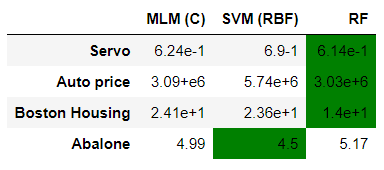
\includegraphics[width=\textwidth]{regr1.png}
    \end{subfigure}
    \begin{subfigure}[b]{0.5\textwidth}
        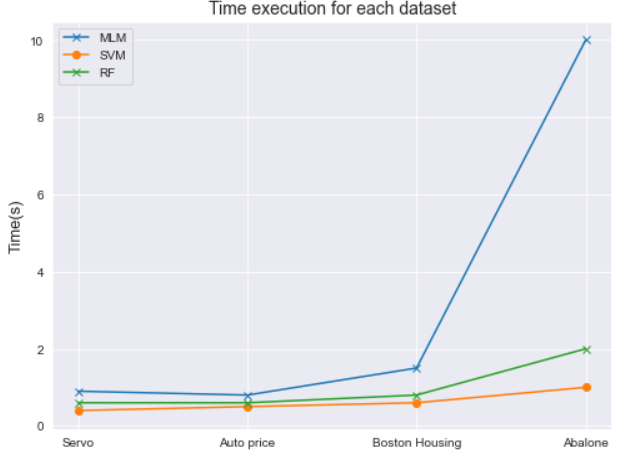
\includegraphics[width=\textwidth]{regr12.png}
    \end{subfigure}
    \caption{MSE results, Time execution}
\end{figure}
 

\par On voit que le RF obtient le meilleur score sur les datasets Servo ,Auto Price et Boston Housing alors que le SVM obtient le meilleur score sur le dataset Abalone. Mais on constate que les résultats du MLM sont très proches des résultats des deux autres méthodes\\
 
\par La figure suivante représente l'évolution de l'erreur en fonction du nombre de références $K$ c'est à dire pour chaque valeur que prend $K$ on calcule le Mean Square Error entre les valeurs prédites et les valeurs réelles ensuite cette valeur est normalisée en la divisant sur le Mean Square Error de ces valeurs prédites.
\begin{figure}[!h]
	\vspace{-0.5cm}
    \centering
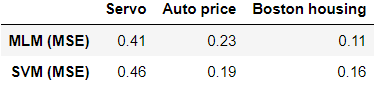
\includegraphics[height=0.4\textwidth]{regr.png}

\end{figure}
\par On voit que les 4 courbes évoluent de la même façon. 

Dans la figure qui suit, on affiche le nombre optimal de points références pour chaque dataset sur 10 différentes exécutions. \\
%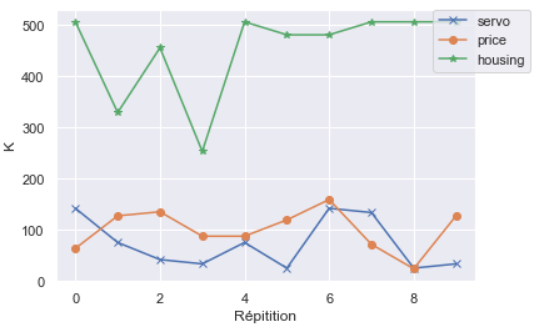
\includegraphics[scale=0.99]{regr3.png}\\
{\color{MidnightBlue}\section{Sur des problèmes de classifications}}
\par Pour la classification on utilise le même processus utilisé pour la régression sauf pour le calcul du taux de précision on utilise l'accuracy.
\begin{figure}[!h]
    \centering
    \begin{subfigure}[b]{0.4\textwidth}
        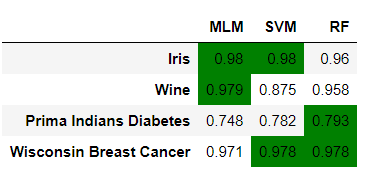
\includegraphics[width=\textwidth]{classif1.png}
    \end{subfigure}
    \begin{subfigure}[b]{0.5\textwidth}
        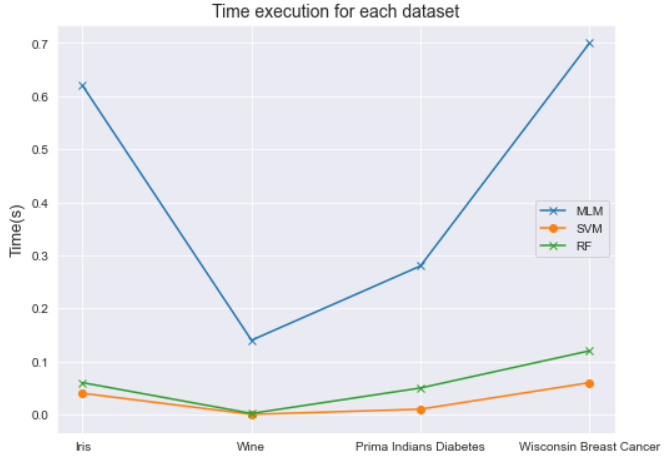
\includegraphics[width=\textwidth]{classif12.png}
    \end{subfigure}
    \caption{Accuracy results, Time execution}
\end{figure}
 
\par Le Minimal Learning Machine obtient le meilleur score pour le dataset Wine et Iris, le SVM est meilleur sur les dataset Iris et Wisconsin Breast Cancer et les RF sont meilleurs sur les deux datasets Prima Indians Diabetes et Wisconsin Breast Cancer\\
\par L'évolution de l'erreur en fonction du nombre de points références:\
\par Le nombre optimal de points références pour les trois datasets Breast Cancer, Iris et Wine sur 10 différentes exécutions: \\

\begin{figure}[!h]
\vspace{-0.5cm}
    \centering
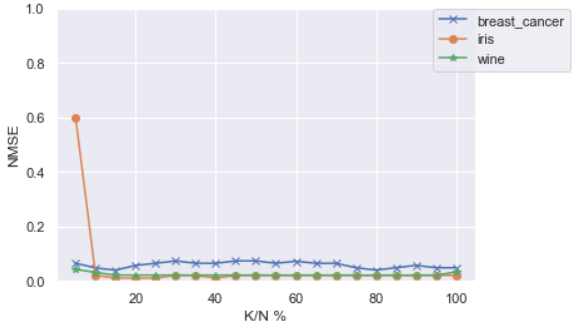
\includegraphics[height=0.4\textwidth]{classif2.png}
\caption{Optimal K value over different runs}
\end{figure}
\par Comme c'est difficile de faire des tests sur des données réelles car l'exécution peut prendre énormément de temps, surtout pour optimiser les hyper paramètres, avec une validation croisée ou une recherche en grille. Donc trois nouveaux ensembles de données de 100 observations à deux dimensions pour 500 instances sont générés, pour comparer les performances du Minimal Learning Machine au SVM et RF. Les données sont près traitées toujours de la même façon.
\par Les trois datasets sont générer aléatoirement en utilisant les fonction "make classificatio","make moons" et "make circle".\\

\par Les trois modèles n'ont pas été optimisé, le nombre de points références est fixé à 0.3 pour le MLM pour le SVM et RF on utilise aussi les valeurs des paramètres par défaut.

Les données sont près traitées de la même façon que dans la section précédente. 
\par Les résultats des trois modèles sont affichés dans ce tableau :\\
\begin{figure}[!h]
    \centering
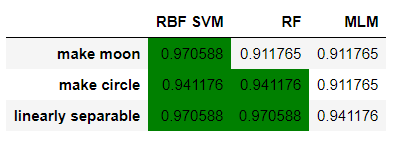
\includegraphics[height=0.2\textwidth]{three_c.png}
\caption{Accuracy score for SVM,RF and MLM}
\end{figure}
\par On voit que les SVM et RF obtiennent les meilleurs résultats mais l'écart avec les résultats du MLM n'est pas grand.

\par Pour montrer l'influence du nombre de points référence utilisé sur la complexité de l'algorithme, on test le MLM sur des données générées aléatoirement avec la fonction "make regression" avec 500 instances pour 5 features, on compte le temps d'exécution sur les mêmes données en utilisant un nombre de points références qui vas de 5\% à 100\% de la taille des données avec un pas de 5\%.

\begin{figure}[!h]
\vspace{-0.5cm}
    \centering
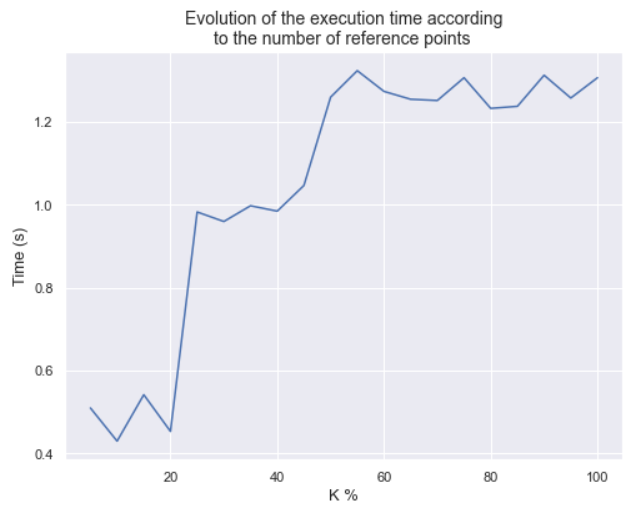
\includegraphics[height=0.45\textwidth]{timeEvol.png}
\caption{Time evolution per K}
\end{figure}
Comme attendu la complexité augumente fortement en parallèle au nombre de références, mais ce n'est pas grave du moment qu'à l'étape de prédiction le processus est rapide.

{\color{MidnightBlue}\chapter{Implémentation d'une version pré calculé}}
\par Maintenant l'objectif est de réussir à implémenter une version pré calculé de la méthode. Le terme \textbf{"pré calculé"} veut dire que dans cette version on donne au modèle les matrices de distances près calculés, directement lors de la formation et aussi lors de la prédiction, ainsi on peut définir notre propre manière de calcul des dissimilarités et donner au modèles les matrices prêtes à être utiliser directement.

\par Avant de pouvoir modifier le code de la méthode, il fallait d'abord coder notre propre version en suivant la procédure décrite dans l'article pour s'approprier la méthode et pouvoir la modifier plus facilement en cas de besoin.

\par La classe principale de la méthode s'appelle MLM, en plus du constructeur elle contient trois parties essentielles, une partie pour la sélection de points références et calcul des matrices de distances, une partie pour la formation du modèle et calcul de la matrice des poids et une partie pour la prédiction et optimisation de la fonction de coût. Pour la classification le même processus est utilisé seulement on transforme d'abord les labels avec \textbf{one hot encoding}. 

\par Après avoir coder la version pré calculé du Minimal Learning Machine, on l'a testé sur les datasets précédemment utilisés avec la même mesure de distance pour  vérifier qu'on retrouve bien les mêmes résultats. Ensuite à l'aide de la fonction \textbf{cdist} de scipy on calcule les matrices de distances avec différentes mesures et on compare avec les résultats obtenus en utilisant la distance euclidienne. Une explication des mesures utilisés est donné ici :
\begin{itemize}

\item La distance \textbf{Caneberra} entre deux points $u,v$ : $ d(u,v) = \sum_i{\frac{|u_i - v_i|}{|u_i| + |v_i|}}$
\item La distance \textbf{chebyshev} entre deux points $u,v$ : $ d(u,v) = max_i{|u_i - v_i|}$ 
\item La distance \textbf{cityblock} entre deux points $u,v$ : calcul la distance de Manhattan 
\item La distance \textbf{sqeuclidean} entre deux points $u,v$ : $ d(u,v) = ||u-v||_2^2$ 

\par On a testé le Minimal Learning Machine sur les 8 datasets précédemment utilisés, les données ont été pré traité de la même façon que dans la partie Expérimentations. Pour chaque mesure de distance sur chaque dataset une cross validation de 5\% à 100\% de la taille des données avec un pas de 5\% pour optimiser le nombre de points références. Pour la régression on utilise le MSE et pour la classification on utilise l'Accuracy comme métriques, les résultats sont affiché dans les figures 4.1 et 4.2 . 
\end{itemize}

\begin{figure}[!h]
  \begin{center}
    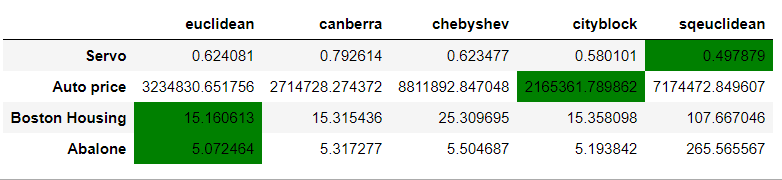
\includegraphics[width=0.8\textwidth]{regr_distances.png}
  \end{center}
  \caption{Regression results (MSE)}
\end{figure}

\begin{figure}[!h]
  \begin{center}
    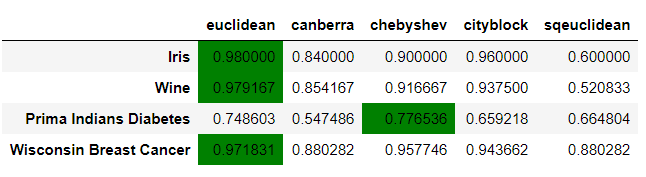
\includegraphics[width=0.8\textwidth]{classif_distances.png}
  \end{center}
  \caption{Classification results (Accuracy)}
\end{figure}
\par Avec la distance euclidienne le MLM obtient le meilleur score pour les datasets Boston Housing et Abalone. Les distances sqeueclidienne et cityblock permettent d'avoir les meilleurs résultats pour les datasets Auto price et Servo. 
Pour la classification la distance euclidienne donne le meilleur score pour les dataset Iris, Wine et Wisconsin Breast Cancer tandis que chebyshev donne le meilleur résultat pour le Prima Indians Diabetes. \
En général la distance euclidienne permet d'avoir de bons résultats sur la plupart des problèmes, néanmoins sur certains problèmes d'autres mesures de distances sont meilleures.
 
{\color{MidnightBlue}\chapter{Minimal Learning Machine avec Random Forest}}
\par Il y a plusieurs façons de calculer des dissimilarités en machine learning, la plus connue d'entre elles est la distance euclidienne. Notre objectif est d'implémenter notre propre version de la méthode Minimal Learning Machine en utilisant les Random Forest pour calculer les dissimilarités, ensuite de comparer les résultats obtenus avec cette méthode aux résultats du Minimal Learning Machine, SVM et Random Forest.

{\color{MidnightBlue}\section{Forêt aléatoires}}
\par Les forêts aléatoires font partie des techniques d'apprentissage automatique, qui combinent les concepts de sous-espaces aléatoires et de \textbf{bagging}.L'idée est de créer plusieurs copies d'un même modèle dans notre cas un arbre de décision, en entrainant chaque copie sur une partie aléatoire du dataset. Pour ça on utilise une technique d'échantillonnage appelé \textbf{Bootstrapping} et qui consiste à replacer après chaque tirage au sort les données qui ont été sélectionné dans notre dataset, de cette manière on obtient une foule de modèles diversifiés puisque il n'ont pas été nourri sur les mêmes données mais qui partagent quand même certaines connaissances en commun, avec ça on regroupe les résultats de chaque modèle pour faire une prédiction final.

{\color{MidnightBlue}\section{Arbre de décision}}
\par Un arbre de décision est une méthode de machine learning ou l'on construit un arbre sur les données d'apprentissages, chaque nœud interne décrit un test sur une variable d'apprentissage, chaque branchement représente un résultat du test et chaque feuille contient la valeur de la variable cible (une étiquette de classe pour les arbres de classification, une valeur numérique pour les arbres de régression).


{\color{MidnightBlue}\section{Calcul de dissimilarité}}
\par Les Random Forest présentent une mesure de similiarité pour une paire d'instances $x_i$ et $x_j$ qui prend en compte les labels correspondant $y_i$ et $y_j$ à l'inverse de la distance euclidienne par exemple qui prend en compte uniquement les deux instances $d(x_i,x_j)=\sqrt{\sum_{k=1}^d (x_i^{(k)} - x_j^{(k)})^2}$.\
On dit que $x_i$ et $x_j$ sont similaire si elles sont proches l'une de l'autre, mais aussi si elles appartiennent à la même classe. $x_i$ et $x_j$ sont similaire si elles suivent le même chemin dans l'arbre de décision. \

\begin{itemize}
	\item On définit l'ensemble de feuille $L_k$ dans $h_k$
	\item soit $l_k : X \rightarrow L_k$ une fonction qui attribue à chaque 					$x$ une prédiction c'est à dire une feuille de l'ensemble $L_k$.
	\item Dans la figure qui suit $l_k(x_i) = N_{12}$
\end{itemize}
\begin{figure}[!h]
    \vspace{-0.9cm}

	\centering
    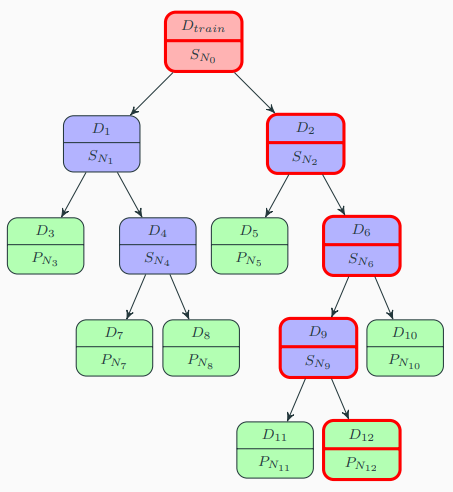
\includegraphics[height=0.5\textwidth]{tree_path.png}
     \caption{Path from root to leaf}
\end{figure}


La similarité $d^{(k)}(x_i,x_j)$ entre $x_i$ et $x_j$ donné par $h_k$ est
$ d^{(k)}(x_i,x_j) = \begin{cases} 1 & \text{if} l_k(x_i) = l_k(x_j)\\ 0 & \text{otherwise} \end{cases} $\
\begin{itemize}
\item La figure (a) représente le cas ou $x_i$ et $x_j$ tombent dans la même feuille $ d^{(k)}(x_i,x_j) =1$
\item La figure (b) représente le cas ou $x_i$ et $x_j$ ne tombent pas dans la même feuille donc $ d^{(k)}(x_i,x_j) = 0$
\end{itemize}

\begin{figure}[!h]
    \centering
    \begin{subfigure}[b]{0.45\textwidth}
        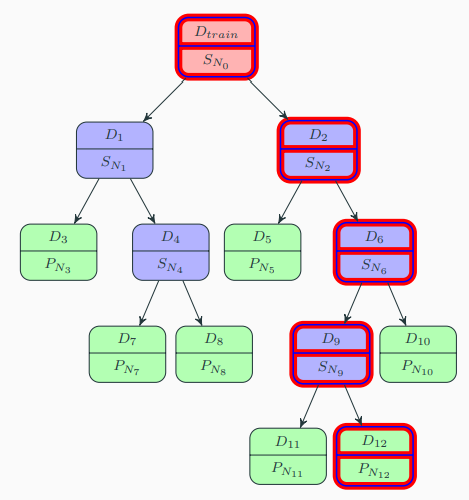
\includegraphics[height=0.99\textwidth]{dissi_1.png}
        \caption{$d^{(k)}(x_i,x_j) = 1$}
    \end{subfigure}
    \begin{subfigure}[b]{0.45\textwidth}
        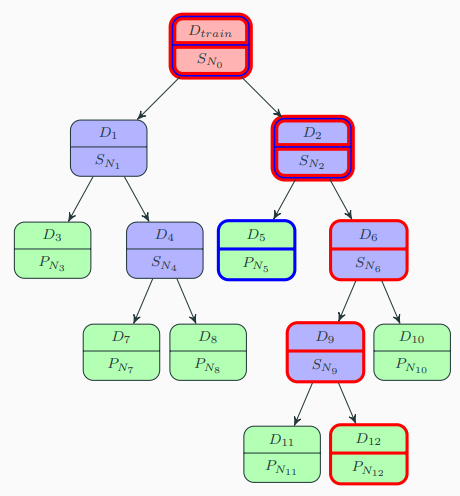
\includegraphics[height=0.99\textwidth]{dissi_0.png}
        \caption{$d^{(k)}(x_i,x_j) = 0$}
    \end{subfigure}
    
\end{figure}


{\color{MidnightBlue}\section{Comparaison des résultats }}
\par  Comme cette version du MLM lance un Random forest à l'intérieur et derrière lance aussi un Minimal Learning Machine, la première question qui nous vient à l'esprit c'est est ce qu'on combinant les deux modèles on obtient de meilleurs résultats qu'avec chaque modèle séparément. Donc pour comparer les résultats des trois modèles on les a testés sur les 8 datasets utilisés précédemment. Les données ont été traité en suivant le même protocole expliqué dans la partie 3 Expérimentations. Concernant les modèles pour une comparaison équitable,pour le Minimal Learning Machine on prend le nombre de points références égale au nombre de données et comme mesure de distance on prend la distance euclidienne. Le Random Forest on le laisse avec les paramètres par défauts donc le nombre d'estimateurs = 100. Le Minimal Learning Machine avec Random Forest dissimilarités prend les mêmes valeurs des paramètres que pour ces deux modèles.


\begin{figure}[!h]
    \centering
    \begin{subfigure}[b]{0.44\textwidth}
        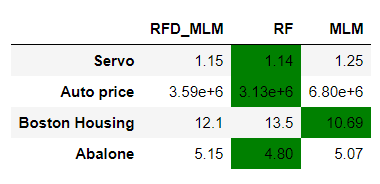
\includegraphics[width=\textwidth]{rfd_regr.png}
         \caption{Regression results (MSE)}

    \end{subfigure}
    \begin{subfigure}[b]{0.46\textwidth}
        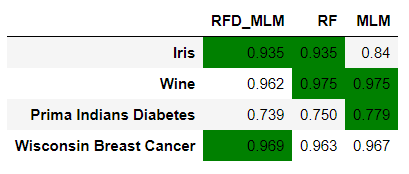
\includegraphics[width=\textwidth]{rfd_classif.png}
        \caption{Classification results (Accuracy)}
    \end{subfigure}
    \caption{Comparison between RF, RFD-MLM, MLM}
\end{figure}



\par On voit que le Random Forest seul obtient le meilleur score sur 3/4 des datasets pour la régression et aussi sur 2/4 des datasets pour la classification. Le MLM avec Random Forest dissimilarités est meilleur sur 2/3 des datasets pour la classification tant dis que le Minimal Learning Machine est meilleur sur 2/4 des problèmes de classification et 1/4 des problèmes de régression.

\par On voit que le Random Forest tout seul reste meilleur que le Minimal Learning Machine ou en combinant les deux. Néanmoins la différence entre les résultats n'est pas très grande entre les trois modèles et surtout entre le RF et RFD-MLM et d'ailleurs en voit qu'en moyenne le RFD-MLM est meilleur que le MLM.  

{\color{MidnightBlue}\section{Comportement du MLM et RF dans des espaces à grandes dimensions}}
\par On teste le Minimal Learning Machine et RFD-MLM sur deux problèmes joués, un pour la régression et un autre pour la classification. Les données sont générées aléatoirement en utilisant les fonctions \textbf{make classification} et \textbf{make regression} de sklearn, pour la classification on fixe les paramètres (n-classes=3,n-informative=2) pour la régression on fixe les paramètres (n-informative=2). Sur chaque un des cas on teste les deux modèles sur 30 tirages aléatoires mais on incrémente le nombre d'instances de 400 et le nombre de features de 40 donc après chaque tour sur 30 itérations. Les deux paramètres varient de 400 à 12000 et de 40 à 1200 respectivement. Pour chaque test les données sont divisées en deux ensembles 2/3 pour le train et 1/3 pour le test, ensuite on standardise les données avec la moyenne et l'écart type des données d'entrainements. Pour la classification les proportions des classes ont été équilibrées.\
Les figures (a) (b) montrent les résultats du test en régression et classification.

\begin{figure}[!h]
    \centering
    \begin{subfigure}[b]{0.45\textwidth}
        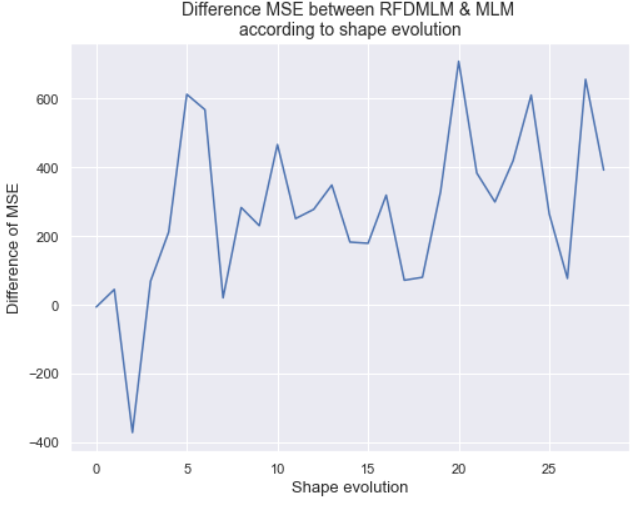
\includegraphics[width=\textwidth]{shapeEvo_r.png}
         \caption{Regression results (MSE)}

    \end{subfigure}
    \begin{subfigure}[b]{0.46\textwidth}
        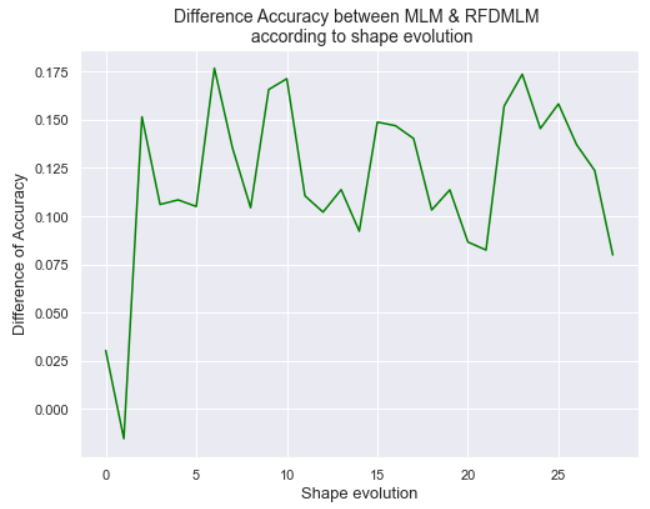
\includegraphics[width=\textwidth]{shapeEvo_c.png}
        \caption{Classification results (Accuracy)}
    \end{subfigure}
\end{figure}

\par On voit que la différence entre les deux résultats est petite au début car les deux modèles donnent des résultats très proches au début avant la cinquième itération ce qui correspond au plages 400 à 2000 instance et 40 à 200 features. A partir de là la différence devient plus grande, alors les résultats du RFD-mlm ne changent pas en moyenne c'est les résultats du MLM qui baissent par exemple en classification sur les 5 premières itérations la moyenne des scores du MLM est 0.86 et sur les 5 itérations suivantes la moyenne est 0.81 alors que pour le RFD-MLM on passe de 0.89 à 0.87.

\par Les résultats montrent clairement que les mesures de distances se comportent mal en grandes dimensions ce qui n'est pas le cas pour les Random Forest dissimilarités.
{\color{MidnightBlue}\chapter{Conclusion et perspectives}}
\par On a vu que le Minimal Learning Machine présente des résultats assez bons en utilisant la distance euclidienne comme mesure de dissimilarité, néanmoins ces performances n'égalent pas celles des SVM et RF. Mais ça reste une méthode de machine learning qui présente des avantages et des inconvénients et qui peut se révéler être un atout pour résoudre certains problèmes. 
\par La nouvelle version de la méthode qui utilise les RF dissimilarités présente beaucoup d'avantages à savoir que ces performances ne changent pas que ce soit en petites ou grande dimension. Et on a vu qu'elle présente des résultats encourageant si on la compare au Minimal Learning Machine, mais ces résultats demeurent moins bon comparés aux résultats des Random Forest. Mais on a beaucoup d'idées pour améliorer le RFD-MLM, en commençant par optimiser le nombre de point référence qui permettra d'un coté de réduire sa complexité et peut être améliorer ces performances.

\par On peut aussi optimiser le RF utilisé à  l'intérieur en commençant par augmenter le nombre d'estimateurs. On a la possibilité d'utiliser d'autre mesures de distances pour les données en sortie, on pourrait même penser à une façon de calculer les dissimilarités pour les données en sortie en utilisant les Random Forest.

\par En plus il y a des variantes du Minimal Learning Machine dont on n'a pas parlé dans ce projet, par exemple il y a une version qui s'appelle OS-MLM (Optimal Selected Minimal Learning Machine) qui au lieux de sélectionner aléatoirement les références des données, choisit de sélectionner certaines données en particuliers, ainsi on pourrait éviter de sélectionner des outliers par exemple ou dans le cas de la classification on pourrai veiller  à sélectionner la même proportions de points références pour chaque classe. Il y a aussi une variante qui s'appelle NN-MLM(Nearest Neighbors Minimal Learning Machine) qui se base sur une approche au plus proche voisin. Donc voilà il y a pleins d'améliorations possibles qu'on pourrait ajouter au RFD-MLM.


{\color{MidnightBlue}\chapter*{Références}}
\par @article{ICML,
    author  = "Cortes, C, Mohris, M. Weston, J.",
    title   = "A general regression technique for
learning transductions",
    year    = "2005",
    journal = "Proceedings of the 22Nd International Conference on Machine Learning.",
    pages   = "153--160"
}
\par @misc{scikit-mlm,
    author       = "Madson Luiz Dantas Dias",
    year         = "2019",
    title        = "scikit-mlm: An implementation of {MLM} for scikit-learn framework",
    url          = "https://github.com/omadson/scikit-mlm",
    doi          = "10.5281/zenodo.2875802",
    institution  = "Federal University of Cear\'{a}, Department of Computer Science" 
}

\par Liens vers l'article MLM : https://www.sciencedirect.com/science/article/abs/pii/S0925231215003021?via\%3Dihub

\par Liens vers Distance Mesures Data : https://towardsdatascience.com/9-distance-measures-in-data-science-918109d069fa
\end{document}
